\documentclass{article}
\usepackage{fullpage}
\usepackage{amsmath,amssymb}
\usepackage{natbib}
\usepackage{marginnote}
\usepackage{graphicx}
\usepackage{color}
\usepackage{hyperref}
\usepackage{latexml} % for \iflatexml

% \newcommand{\var}{\mathop{\mbox{Var}}}
% \newcommand{\Exp}{\mathop{\mbox{Exp}}}
\DeclareMathOperator{\var}{Var}
\DeclareMathOperator{\Exp}{Exp}
\DeclareMathOperator{\sn}{sn}
\renewcommand{\P}{\mathbb{P}}
\newcommand{\E}{\mathbb{E}}
\newcommand{\R}{\mathbb{R}}
\newcommand{\calE}{\mathcal{E}}
\newcommand{\calC}{\mathcal{C}}
\newcommand{\dconv}{\xrightarrow{d}}
\newcommand{\deq}{\stackrel{\scriptscriptstyle{d}}{=}}

\newcommand{\migrate}{\lambda_\text{mig}}
\newcommand{\mutrate}{\lambda_\text{mut}}
\newcommand{\Tmig}{T_\text{mig}}
\newcommand{\Tmut}{T_\text{mut}}

\newcommand{\gc}[1]{{\it\color{green}(#1)} }
\newcommand{\plr}[1]{{\it\color{blue}(#1)}}

\bibliographystyle{plainnat}

\begin{document}

\section{Introduction}

The covergent evolution of similar phenotypes in response to shared
selection pressures is a testiment to the power of selection to
repeatedly sculpt phenotypic variation. 
In some cases this convergence extends to the molecular level with
dispate taxa converging to the same phenotype through parallel genetic
changes in the same pathway, genes, 
or even by precisely the same genetic changes \citep{zhen2012parallel}. 
Such precise convergence points to the conservation of function of the genes
underlying adaptive traits, 
sometimes over deep time scales \citep{deephomologypapers}. 
Convergence on a molecular level also suggests that the path 
accessible to adaptation is sometimes relatively constrained, 
as would be the case if only a few changes confer the advantagous phenotype 
and are sufficiently free of deleterious pleiotropic consequences.

%For highly polygenic traits 

Convergent adaptation can also occur within species, if individuals within a species 
adapt to the same environment, in parallel, through different genotypic changes. 
There are a growing number of examples of this in a range of well studied organisms and phenotypes REFs.
All else being equal, such evolution of convergent phenotypes is more likely with a 
higher mutational input, that is, when the mutational target and population sizes are larger \citep{}. 
The geographic distribution of populations can also affect the probability of parallel mutation within a species:
a widespread species is more likely to adapt by multiple, parallel mutations if dispersal is geographically limited, 
since subpopulations will adapt via new mutations before the adaptive allele arrives via migration \citep{ralph2010parallel}. 
Standing variation for a trait can also increase the probability of convergence, 
and standing variation for an allele increases the probability that the selective sweep will be \emph{soft}
(beginning from a base of multiple copies),
leading to genetic patterns similar to convergent adaptation \citep{orr2001sieve,softsweepsI}. 

Intuitively, convergence is also more likely 
when geographically separated populations adapt to ecologically similar conditions. 
The probability that convergent adaptations arise independently
before adaptations spread between the populations by migration
will be larger if these adaptive alleles are maladapted in intervening environments,
since such adverse conditions can strongly spatially restrict the spread of locally adapted alleles \citep{slatkin1973geneflow}.
 
One elegant set of such examples is provided by the assortment of plant species 
that have repeatedly adapted to patches of soil with high concentrations of heavy metals
(e.g.\ serpentine outcrops and mine tailings) \citep{turner2010serpentine,mimulus};
the alleles conferring heavy metal tolerance are thought to be locally restricted 
because they incur a cost off of these patches. 
Similarly, across the American Southwest, a variety of species of animals have developed locally adaptive cryptic coloration
to particular substrates, e.g.\ dark rock outcrops or white sand dunes \citep{benson1933concealing}.
One of the best-known examples is the rock pocket mouse (\textit{Chaetodipus intermedius}),
which is primarily dark on a number of black lava flows separated by much lighter soil \citep{dice1940ecologic}.
Strong predator-mediated selection appears to favour such crypsis \citep{kaufman1974adaptive},
and, perhaps as a result of this strong selection against migrants, 
at least two distinct genetic changes are responsible from the dark pigmentation adaptation on different outcrops \citep{nachman2003different}. 
Similar situations have been demonstrated in other small rodent systems \citep{steiner2009genetic,kingsley2009melanism}.

In this paper, we study this situation, namely,
when a set of alleles provide an adaptive benefit in geographically localized patches, 
separated by (inhabited) regions where the alleles are deleterious.
\plr{or neutral?}
The main questions are:
Under what conditions is it likely that each patch adapts in parallel, through new mutation,
and when is it likely that migration carries these alleles between patches?
How could we tell, after the fact, which has occurred?
We work in a model of continuous geography,
using a variety of known results and new methods.
In section XX we \dots QUICK OUTLINE


%http://www.nature.com/hdy/journal/v94/n2/full/6800600a.html


%and that a single mutational change was sufficient to adapt populations to the novel environment. 
%We assumed that there was no standing variation for the adaptive allele, such that parallel mutation must be due to multiple mutations after the environmental shift. In that setting we found that there was a characteristic geographic scale, over which we would expect multiple instances of our adaptive allele to have arisen in parallel. This characteristic length could be expressed in terms of a simple compound parameter determined by our parameters of interest.
%Recall questions of origin of adaptations

%References on parallel adapation, standing variation, etc.:
 % coop,
 % pennings and hermisson.
%Note pennings and hermisson found standing deleterious variation was very important.  

%recall peromyscus examples with patchy environments

%Summarize previous paper

%Question assumptions of no standing variation and homogenous selection


%%%%%%%%%%%%%
\section{Methods}

%%%
\subsection{Model of a patchy landscape}
\label{ss:patchyspace}

Consider a population spread across a landscape, 
within which are patches of habitat to which individuals are (initially) poorly adapted,
surrounded by large areas to which the population is well adapted.
(When we refer to ``patches'' it is to these pieces of habitat.)
Suppose it takes only a single mutational change to create an allele ($B$) that adapts an individual to the poor habitat type, 
a change that occurs at a (low) rate of $\mu$ per chromosome per generation. 
We assume that this initially rare new
allele has fitness $1+s_p$ relative to the unmutated type ($b$) in these ``poor'' habitat patches,
and assume that it has fitness $1-s_m$ when rare in the intervening areas, with $s_p, s_m > 0$.
To simplify matters, we assume that the disadvantage $s_m$ 
is sufficiently large that, on the relevant timescale,
the allele is very unlikely to fix locally in the regions where it is at a disadvantage.
(The case where $s_m=0$ requires a different approach, which we do not treat here.)

We are interested in the establishment of mutations in the ``poor'' patches by either
migration or mutation, and so are mainly interested in whether the allele
can escape initial loss by drift when rare. 
Therefore, we do not have to specify the the fitness of the homozygote; 
only that the dynamics of the allele when rare 
are determined by the fitness of the heterozygote. 
More general dominance will only make small corrections,
with the exception of the recessive case, which we omit.
For the most part, 
we follow the literature in treating the diploid model as essentially haploid.

For the sake of simplicity, we assume a constant haploid population density $\rho$, 
across both types of habitat (we return to discuss this equal density point later). 
We further assume that the variance in offspring number is $\xi^2$, 
and that the mean squared distance between parent and child is $\sigma^2$
(i.e.\ $\sigma$ is the dispersal distance).
We also aim to describe the scenario where it is sensible to think of large, discrete patches;
the case of a fine-scale hetergeneous environment is treated \citep{elsewhere}.

\paragraph{Previous work} 
We will make use of several previous results from the literature. 
XXX cite nagylaki 1974: does 2d clines XXX
\citet{haldane1948theory}, working with the one dimensional partial differential equation,
showed that with large patches, the spatial scale over which the two types intergrade is given by $\sigma/\sqrt{s}$,
with $s$ either $s_m$ or $s_p$ as appropriate.
\citet{slatkin1973geneflow}, in the same setting,
showed that if the physical width of the patch is less than $2 (\sigma/\sqrt{s_p}) \tan^{-1} (\sqrt{s_m/s_p})$, 
then there is no stable equilibrium with both $b$ and $B$ present,
so that migrational swamping prevents $B$ from establishing \citep[see also][ for a review]{lenormand2002limits}.
\citet{barton1987establishment}, using general theory of \citet{pollak1966survival}, showed (again in one dimension) 
that this critical patch size also holds in a stochastic framework.
\citet{barton1987establishment} also showed that
for patches above this critical size,
the probability of establishment of a new mutant that appears at distance $r$ from the patch
decays exponentially with distance from the patch, with the scale given by $\sigma/\sqrt{s_m}$,
and that mutations appearing within the patch have probability of establishment
less than the probability for a panimictic population,
but approaching this as the size of the patch increases.
(This latter panmictic probability of establishment we denote $p_e$,
and often approximate by $2 s_p / \xi^2$ \citep{haldane,fisher}.)
This result holds quite generally for a geographically spread population that experiences a uniform selection
pressure \citep{maruyama1970fixation,cherry2003diffusion}. 



%%%%%
\subsection{Establishment of a locally adaptive allele due to mutational influx}
\label{ss:patchymutation}

Consider first a single, isolated poor habitat patch of area $A$ in which no $B$ allele has yet become established. 
We first compute the time scale on which new $B$ mutations appear and fix in such a patch.
As we are interested in patches where local adaptation can occur,
we will assume that our patch is larger than the cutoff for local establishment, 
i.e.\ wider than $2 \tan^{-1} (\sqrt{s_m/s_p})$ \citep{slatkin1973geneflow}.

Let $p(x)$ be the probability that a new mutant $B$ allele arising at location $x$ 
relative to the patch fixes within the poor habitat patch.
As shown in Appendix \ref{apx:eqfreq},
the function $p(x)$ can be found (in one dimension) in terms of Jacobi elliptic functions,
but the precise expressions are not particularly helpful.
The total successful mutational influx per generation is then given by the integral of $p(x)$ over the entire species range,
% $\int \rho \mu p(x) dx$,
and hence depends in a complicated way on the relationship of patch width and selection coefficients,
but still scales linearly with the mutational influx density $\rho \mu$.
If the width of the patch is large relative to $\sigma/\sqrt{2s_m}$, 
then a reasonable approximation is to assume that $p(x) = p_e$ within the patch, and $p(x) = 0$ otherwise,
for a patch of area $A$ approximating $\int p(x) dx \approx 2 s_p A / \xi^2$. 
This holds for large patches, in which the rate at which mutations arise within the patch is larger 
than the rate at which they appear nearby;
we examine this more generally via simulation in Appendix \ref{apx:establishment_sims}.

The rate at which mutations arise and colonize a patch of area $A$ is therefore
\begin{align} \label{eqn:mutrate}
  \mutrate = \rho \mu \int p(x) dx  \approx 2 s_p \rho A \mu / \xi^2.
\end{align}
If this rate is low, then the time (in generations) until a mutation arises that
will become locally established within the patch is exponentially distributed with mean $1/\mutrate$.  
Assuming that once a mutation becomes established it quickly reaches its equilibrium frequency across the patch, 
the time scale on which new patches become colonized by the $B$ allele from new mutation is therefore approximately $1/\mutrate$.


%%%%%%%
\subsection{Establishment of a locally adaptive allele due to migrational influx}
\label{ss:patchymigration}

Now suppose that there are two patches, each of area $A$ and separated by distance $r$. 
If the $B$ allele has arisen and become established in the first patch, but has not yet appeared in the second,
we would like to know the time scale on which copies of $B$ move between patches by migration
(so, ignoring the possibility that a $B$ allele arises independently by mutation in the first patch).
To determine this, we dissect the process by which an allele transits between the patches,
in the process obtaining other useful information about the genealogy.

\begin{figure}[ht!]
  \begin{center}
    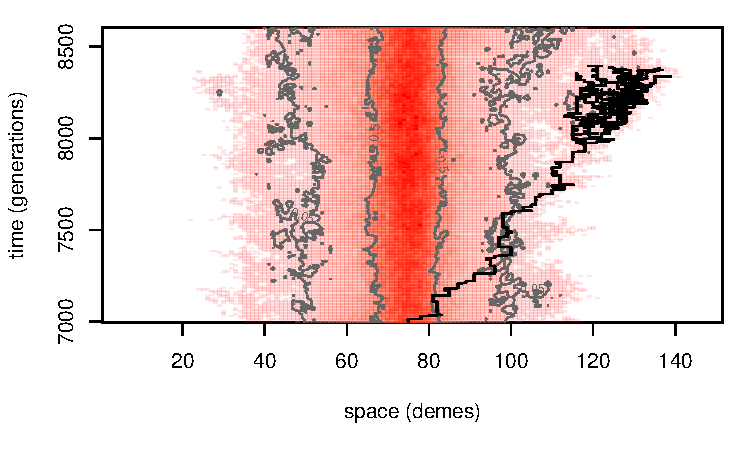
\includegraphics{sim-snapshots}
  \end{center}
  \caption{
  Results from individual-based simulation, on a one-dimensional grid:
  the focal allele is beneficial in the central 20 demes, with $s_b=0.1$,
  and deleterious elsewhere, with $s_m=-0.02$.
  The dynamics were simulated for 10000 generations; demes had 1000 individuals in each;
  dispersal was to nearby demes with a mean dispersal distance of $\sigma \approx 1.66$  times the deme spacing.
  \textbf{(A)} Allele frequencies across space: colored lines are snapshots at an evenly spaced set of times,
  and the solid lines shows the cumulative mean occupation frequency across all generations.
  \textbf{(B)} A segment of the temporal dynamics: space is again shown across the horizontal axis;
  with time on the vertical axis; demes are colored darker red the greater then allele frequency at the corresponding time.
  The 50\% and 5\% frequency contour lines are in grey,
  and the genealogy of 50 individuals in a rare long-distance excursion is traced back with black lines.
  \label{fig:sim_snapshots}
  }
\end{figure}

Migration--selection balance ensures that 
there will be some number of $B$ alleles present in the regions where they are disadvantageous,
but only very few, and rarely, far away from the patch where $B$ is established.
Denote the expected frequency of allele $B$ at distance $r$ from the patch by $q(r)$.
Following \citet{slatkin1973geneflow}, one can write down a differential equation to which $q(r)$ is the solution,
which can then be solved to give $q(r)$ in terms of Jacobi elliptic functions (see Appendix \ref{apx:elliptic_integrals}).
Asymptotics of these implies that for large $r$ the mean occupation frequency decays exponentially, 
\begin{align} \label{eqn:eqfreq}
    q(r) \approx C \exp( - r \sqrt{2 s_m} / \sigma) \qquad \text{for large $r$},
\end{align}
where $d$ is the dimension ($d=1$ or $2$), and $C$ is a constant depending on the geographic shape of the populations and the selection coefficients. 
In Appendix \ref{apx:patchy_sims} we argue that $C=1/2$ is about right for most parameter values,
and also that these asymptotics are correct in both one and two dimensions
(the differential equation is only analytically solvable in one dimension).

This expected frequency $q(r)$ is the \emph{time-averaged} occupation frequency,
or in other words, the total number of $B$ alleles found at distance $r$ across $T$ generations, divided by $T$.
Therefore, if we look at a small area of size $\epsilon$, 
then $q(r) \epsilon$ is equal to the probability of finding any $B$ alleles there,
multiplied by the mean number of such, if there are any.
This points to an important fact: 
close to the original patch, the ``equilibrium frequency'' $q(r)$ describes well the density of the $B$ allele at most times,
but far away from the patch, there are rare excursions of a family of $B$ alleles, interspersed by long periods of absence.
To compute the rate of establishment by such migration,
we use properties of subcritical branching processes and Brownian motion,
combined with \eqref{eqn:eqfreq},
to obtain an approximation that we argue is valid if the distance $r$ is large relative to $\sigma/\sqrt{s_p}$.

\begin{figure}[ht!]
  \begin{center}
    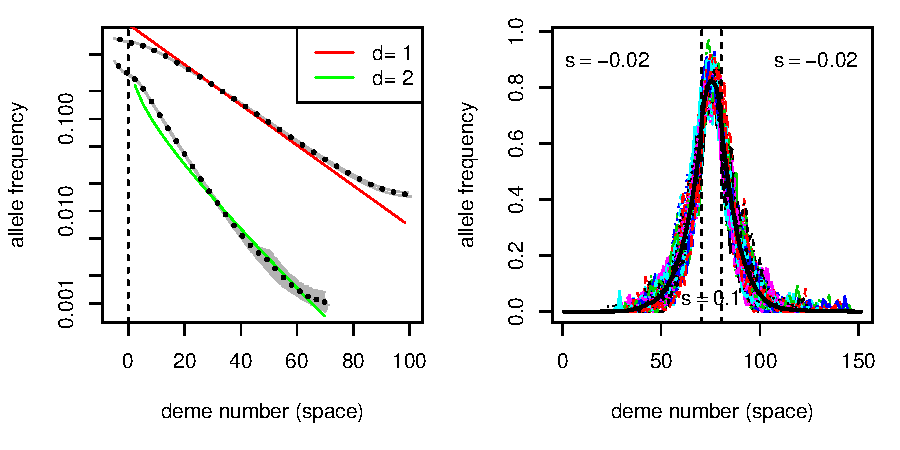
\includegraphics{sim-occupation-freqs}
  \end{center}
  \label{fig:sim_occupation_freqs}
  \caption{
  Mean occupation frequencies from simulation; details are as in figure~\ref{fig:sim_snapshots} except as otherwise noted.
  Each panel shows mean occupation frequencies of individual demes (grey dots)
  and averaged over demes at similar distances (black circles), on
  \textbf{(A)} a one-dimensional grid of 150 demes, and
  \textbf{(B)} a two-dimensional grid of $50\times 50$ demes.
  Superimposed in black is the decay predicted by \eqref{eqn:eqfreq} (with $C=1/2$).
  The two distinct lines of grey points in (A) are to the left and right of the patch, respectively.
  }
\end{figure}

The arguments depends on the following decomposition of the genealogy of $B$ alleles.
First, fix some intermediate distance $r_0$ from the established patch,
and classify all $B$ alleles present at any time outside $r_0$ into families
if they share a common ancestor living outside $r_0$.
If $r_0$ is large enough that there are not too many families
and interactions between family members are weak,
then these families can be approximated by a collection of independent spatial branching processes.
(This can be made formal in the limit of large population density.)
We can extend these families by 
including any individual outside the original patch (but perhaps inside $r_0$) 
that has a parent outside $r_0$,
so that these branching processes are rooted at $r_0$, and are killed upon reaching the original patch.
This decomposition is illustrated in~\ref{fig:sim_snapshots}, and later in figure~\ref{fig:branching_decomp}.
In terms of these families, the equilibrium frequency above is then
\begin{align}
    \label{eqn:gestalt_q}
    \begin{split}
        q(r) &= \text{ ( outflux of families ) } \times \text{ ( mean occupation density of a family at $r$ ) } ,
\end{split}
\end{align}
and the quantity we wish to compute,
the effective rate of at which \emph{families} of migrant $B$ alleles establish in a new patch at distance $r$, 
is
\begin{align}
    \label{eqn:gestalt_migrate}
    \begin{split}
        \migrate(r) &= \text{ ( outflux of families ) } \times \text{ ( probability a family establishes in patch at $r$ ) }
    \end{split}
\end{align}
All terms except the ``outflux of families'' are simple calculations with spatial branching processes;
and we can solve for this outflux using equation \eqref{eqn:eqfreq}.
Here $\migrate$ reflects the mean number of establishing migrant families per unit time,
rather than individuals,
because family establishment events may include more than one individual,
so individual establishment events are clustered in time,
and using their overall density to obtain a typical waiting time until the next event
will underestimate that time.


%%%%
\subsubsection{The genealogy of migrant families}

To understand the process of adaptation by migration,
we therefore need to look more closely at the rare families of $B$ the allele far from the patches where it is established.
Consider one such family.
As noted above, we can model this by assuming that each individual
migrates, then reproduces, independently of all other family members.
The mean squared migration distance is $\sigma^2$, takes the migrant in a random direction,
and if migration takes the individual into a patch where the $B$ allele is favored, 
we drop the individual from our family.
Since the $B$ allele is uniformly deleterious elsewhere,
we can decouple reproduction and migration
by first forming a tree in which each individual has a random number of offspring
(with mean $1-s_m$ and variance $\xi^2$),
then assigning spatial locations to each individual in the tree,
and then pruning any branches that happen to wander into a patch.
This pruning removes both 
branches leading into the new patch (we will need to count these),
and branches leading back into the already established patch 
(which contribute little, since they are going the wrong direction;
so we ignore these).  % but could add detail in appendix

Since each individual has on average $(1-s_m)$ offspring,
a family has on average $(1-s_m)^t$ members in generation $t$.
Let $p_e(t)$ be the chance of extinction by time $t$, and let $K_t$ be the (random) family size conditioned on nonextinction,
so that $(1-s_m)^t = (1-p_e(t))\E[K_t]$.
It turns out that by assuming the fate of each offspring is independent (i.e.\ that this forms a branching process),
and that the distribution of offspring numbers is not too heavy-tailed \citep[see][for details]{jagers1975branching},
that $K_t$ has a limiting distribution: $K_t \dconv K$ 
and that $(1-s_m)^{t}/(1-p_e(t)) \to \E[K]$ as $t \to \infty$.
In other words, the chance of survival to time $t$ is a constant multiplied by $(1-s_m)^t$,
and conditional on survival, the family size is of fixed magnitude.

We can understand this quite concretely, by a method described rigorously by \citet{geiger1999elementary}.
When we condition on survival until $t$, we condition on existence of at least one lineage from time $0$ to time $t$.
Once given this lineage, nothing distinguishes any of the other reproduction events --
each individual in this lineage must give birth to at least one offspring,
and all other reproduction events are unconditioned.
In other words, the genealogy of a family that survives until $t$
can be decomposed into a ``trunk'' that 
sprouts independent ``branches'' that may or may not survive until $t$.
This process is depicted in Figure~\ref{fig:branching_decomp}A.
Concretely, if we write $Z_t$ for the number of offspring in the branching process alive at time $t$
(so $\P\{Z_t = 0\} = p_e(t)$),
then
\begin{align}
  \left( Z_t \; \vert \; Z_t>0 \right) \deq \sum_{s=0}^t \sum_{k=1}^{W_s-1} Z^{(s,k)}_{t-s},
\end{align}
where each $Z^{(s,k)}$ is an independent copy of $Z$,
and each $W_s$ is an independent copy of the offspring distribution, conditioned on $W_s \ge 1$.

\begin{figure}[ht!!]
  \begin{center}
    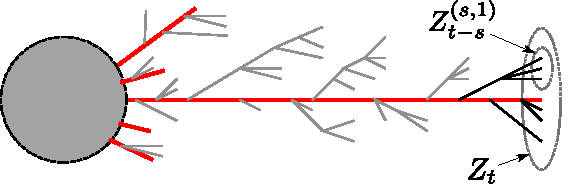
\includegraphics{branching-concept}
  \end{center}
\caption{Cartoon of the decomposition described in the text.
Migrants families are emerging from the already-established patch (grey circle);
each is composed of a ``trunk'' lineage (in red), whose spatial motion we follow,
embellished by transient branches.
For the depicted long-lived family, these are further distinguished by those still alive at time $t$ (in black)
and those that did not survive until $t$ (in grey).
Figure~\ref{fig:sim_snapshots} has a depiction of such a family, from a simulation.
\label{fig:branching_decomp}
}
\end{figure}

This suggests that we will lose little by following only the motion of the ``trunk''
(i.e.\ the red line in figure \ref{fig:branching_decomp}),
and adding the other $K-1$ surviving family members as a cluster about this trunk.
The motion is is approximately Brownian, with variance $\sigma^2$ per generation,
with $\sigma$ is the dispersal distance.
Suppose that the new patch is at distance $r$.
The probability density for the first time such a Brownian motion $B_s$ hits $r$ is
\citep[XXX]{feller}
\plr{work in $d=2$}
% note $\sigma B_t \deq B_{\sigma^2 t}$ so $\P\{ \sup_{s\le t} \sigma B_s \le r \} = \P\{ \sup_{s \le \sigma^2 t} B_s \le r \}
\begin{align} \label{eqn:hitting_dist}
  \P\{ B_t=r \;\mbox{and} \; B_u<r \;\mbox{for all}\; u<t\} =  \frac{r}{\sigma^3 t^{3/2}\sqrt{2\pi}} \exp\left(-\frac{r^2}{2t\sigma^2}\right) .
\end{align}
Let $\tau$ be this random time at which a given migrant family hits the new patch,
with the convention that $\tau =\infty$ if the family never gets here.
We approximate the chance that a given family arrives at the new patch at time $t$, i.e.\ that $\tau=t$,
by the product of equation~\eqref{eqn:hitting_dist} and the probability that the migrant family survives until time $t$.
For convenience, define $\alpha := - \log(1-s_m)$ to be the rate of decrease between patches (note that $\alpha \approx s_m$),
and $\mu_K = \E[K]$ to be the limiting mean family size conditioned on survival,
so that $1-p_e(t) \simeq (1/\mu_K) \exp(-\alpha t)$.
Then, the probability distribution of $\tau$ is given by
\begin{align}
    \P\{ \tau \in dt \} =  \frac{1}{\mu_K} \frac{r}{\sigma^3 t^{3/2}\sqrt{2\pi}} \exp\left(-\frac{r^2}{2t\sigma^2} - \alpha t \right) dt  .
\end{align}

By integrating over~$t$, the chance that this family ever arrives at the new patch is
\begin{align} 
\label{eqn:estab_prob}
  \begin{split}
      \P\{ \tau < \infty \} &= \int_0^\infty \P\{ \tau \in dt \} = \frac{1}{\mu_K} \exp\left( - \frac{ r \sqrt{2 \alpha}}{\sigma} \right) .
  \end{split}
\end{align}
This is, up to the constant $\mu_K$, the chance that a Brownian motion killed at rate $\alpha$
ever hits $r$ \citep{feller}.
This approximation depends on $r$ being large enough so that the approximation $1-p_e(t) \approx (1-s_m)^t/\mu_K$ holds.

Now, each member of a family that successfully arrives at the new patch
(where the $B$ allele is again beneficial)
has a chance $p_e$ of establishing.
The precise distribution of the number of members of a family that enter the patch
given the trunk arrives there
depends on the geometry of the patch,
but since family members should not be too far from the trunk,
we can approximate this by the total size of the family.
If the family has $K$ individuals when the trunk arrives at the new patch,
the chance that any establish is approximately $1-(1-p_e)^K$;
and so that chance that the family establishes, given it arrives at the new patch, 
is 
\begin{align}
    \label{eqn:prob_estab_arrival}
    \E[1-(1-p_e)^K] \approx 2 s_p \mu_K/\xi^2 .
\end{align}

In summary, the probability that an outmigrant from the already-established patch establishes in a new patch at distance $r$ away is 
equal to the probably the trunk arrives (equation~\eqref{eqn:estab_prob}) multiplied by the probability it establishes (equation~\eqref{eqn:prob_estab_arrival}),
namely
\begin{align} \label{eqn:bp_prob_estab}
    F(r) &:= \text{( prob family establishes at $r$ )} = \frac{2s_p}{\xi^2} \exp\left( - \frac{r \sqrt{2 \alpha}}{\sigma} \right) ,
\end{align}



%%%%%
\subsubsection{The rate of outflux of migrant families}

Now, we can obtain the effective ``outflux of families'' from information about the migrant families, combined with \eqref{eqn:gestalt_q}.
Define $\gamma$ to be this outflux; 
i.e.\ the mean number of individuals per unit time whose ancestors carrying the $B$ allele all lived closer than $r_0$ to the original patch
but migrate to a larger distance.
Then for $r>r_0$, the mean occupation density $q(r)$ is equal to $\gamma$ 
multiplied by the mean occupation density of the family descending from such a migrant,
which we denote $u(r)$.
Denote by $Z_t$ the number of individuals such a family has after time $t$,
and the locations of these by $X_1(t), \ldots, X_{Z_t}(t)$.
Then this mean occupation density, at $x$, is the expected number of individuals ever present at $x$. 
Since the expected number of individuals present at time $t$ is $e^{\alpha t}$
and the location of each of these individuals is marginally distributed as a  Gaussian with variance $\sigma^2 t$,
we can write this expectation as
\begin{align}
    u(x) &= \int_0^\infty \E[ \#\{ k : \; X_k(t) \in dx \} ] dt \\
    &= \int_0^\infty e^{\alpha t} \frac{1}{\sqrt{2 \pi t \sigma^2}} e^{-\frac{x^2}{2t\sigma^2}} dt \\
    &= \frac{ 1 }{ \sigma \sqrt{2 \alpha} } \exp\left( - \frac{ x \sqrt{2\alpha} }{ \sigma } \right) 
\end{align}
\plr{check that}
The integral is evaluated in Appendix~\ref{apx:some_integrals}.
\plr{Also examine non-dependence on $r_0$.}

Combining this with the solution for $q(r)$ (equation~\eqref{eqn:eqfreq}) as in \eqref{eqn:q_gestalt},
we then have that (with $C=1/2$)
\begin{align} \label{eqn:outflux}
    \gamma = \text{( outflux of families )} \approx (1/2) \rho \sigma \sqrt{2\alpha} .
\end{align}

Combining this with \eqref{eqn:bp_prob_estab}, as in \eqref{eqn:gestalt_q}, 
the rate of establishment, for a patch of area $A$ at distance $r$ from an already occupied patch, is approximately
\begin{align} \label{eqn:migrate}
    \migrate(r) = \gamma F(r) = \frac{\rho \sigma s_p\sqrt{2s_m} }{\xi^2}  \exp\left( -\frac{ \sqrt{2 s_m} r}{\sigma} \right).
\end{align}
Note that the exponential term is expected based on \eqref{eqn:eqfreq} -- 
since establishment requires rare long distant migrants to be present, and \eqref{eqn:eqfreq} gives the density of such --
but the first term required other arguments.

If this establishment rate is low, 
the time (in generations) before migrant copies of the allele successfully establish through migration in the second patch
is approximately exponentially distributed with mean $1/\migrate$.
Neglecting the time for such a migrant allele to establish once present in the second patch,
the time scale on which migrant alleles transit and fix between patchs is $1/\migrate$.


%%%%%%%%%
\subsection{The probability of parallel adaptation between patches.} 
\label{ss:probparallel}

We now turn to the question of whether the separated populations adapt by parallel genetic changes 
or by the spread of a migrant allele between the patches
(or both, or neither).
As only a single mutation is required for individuals to adapt to the
poor habitat patch, subsequent mutations that arise after an allele becomes established in the patch gain no selective benefit. 
Similarly, an allele introduced into a patch by migration will not be favored by selection to spread, 
if the patch has already been colonized. 
Therefore, mutations selectively exclude each other from patches, over short time scales, 
and will only slowly mix together over longer time scales by drift. 

We will assume that once a $B$ allele is introduced (by migration or mutation), 
it becomes established in the poor habitat patch rapidly. 
Under this approximation, and the ``selective exclusion'' just discussed,
after one of the patches becomes colonized by a single $B$ allele, 
the other patch will become colonized by migration or mutation, but not by both. 
As such, the question of how the the second patch adapts
simply comes down to whether the a new mutation or a migrant allele is the first to become established in the second patch. 

Taking expressions \eqref{eqn:mutrate} and \eqref{eqn:migrate} above,
we see that if the patches each have sufficiently large area,
the rate of migration and mutation will be on the same order if 
$\mu \approx ((s_p+s_m)/2) \exp(-\sqrt{2 s_m} r / \sigma)$,
\plr{check}
where $r$ is the distance between the patches.
(Note that in both cases, $A$ is the area of the not-yet-adapted patch.)

If we take $\mu = 10^{-8}$, and $s_p=s_m=s$, then this is satisfied if $r/\sigma \approx (18+\log(s))/\sqrt{s}$,
so if the selective pressure is fairly strong (say, $s=.05$),
then the distance between patches must be about 70 times the dispersal distance (i.e.\ $r/\sigma \approx 68$);
while if $s$ is much smaller, say $s = .001$, 
then the patches must be separated by many hundreds of times the dispersal distance (i.e.\ $r/\sigma \approx 368$).
The situation does not change much if $\mu$ is larger -- even if $\mu = 10^{-6}$, 
the required separation between patches is only reduced by $5/\sqrt{s_m}$.
If the separation between patches is much larger than this value -- certainly, by a factor of ten -- 
then patches are effectively isolated -- most adaptation will occur independent between patches.
On the other hand, if the separation is much smaller, then a single
mutation is likely to fix in both patches.

One way to visualize this is by a phase diagram.
In figure \ref{fig:phase_diagram},
we give a contour plot for the time until adaptation by migration ($\Tmig = 1/\migrate$) and by new mutation ($\Tmut=1/\mutrate$)
as a function of population density, mutation rate, and distance between patches (scaled by $\sqrt{s_m}/\sigma$).

\begin{figure}[ht]
  \begin{center}
    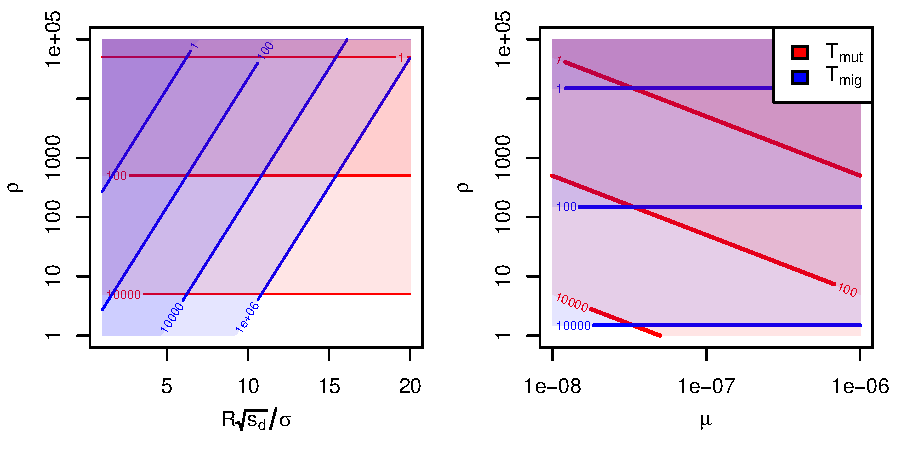
\includegraphics{phase-diagram-log}
  \end{center}
  \caption{
  Mean time until adaptation in a new patch occurs by migration ($\Tmig$, blue) or by mutation ($\Tmut$, red),
  as a function of population density ($\rho$), mutation rate ($\mu$), 
  and distance to an already adapted patch ($R$), scaled by $\sqrt{s_m}/\sigma$.
  Note that population density and mutation rate are shown on a log scale.
  \plr{fix axis labels}
  \label{fig:phase_diagram}
  }
\end{figure}

If we are willing to take these approximations at face value, 
and assuming both rates are small, 
the time until the first of the two patches is colonized by the $B$ allele will be approximately exponentially distributed with mean $1/(2 \mutrate)$.
Following this, the time till the second patch is subsequently colonized 
(via either migration or new mutation) 
will be exponentially distributed with mean $1/(\mutrate+\migrate)$.
Both these times scale linearly with $\xi^2/(\rho A s_{B})$, \plr{check}
so that the overall time to adaptation is robustly predicted to increase with offspring variance ($\xi^2$)
and decrease with patch population size and benefical selection coefficient.
Furthermore, the probability that the second adaptation is a new mutation,
i.e.\ the probability of parallel adapatation, is
\begin{equation}
  \frac{\mutrate}{\mutrate+\migrate} = \frac{2\mu/(s_p+s_m)}{2\mu/(s_p+s_m) + \exp\left(- \sqrt{2 s_m} r / \sigma \right) },
\end{equation}
\plr{check}
so that the probability of parallel mutation should increase
approximately logistically with the distance between the patches, at rate $\sqrt{s_m} /\sigma$. 



%%%%%%%%%%%%
\subsection{Multiple patches}


We can extend this reasoning to multiple patches of unadapted habitat 
in which the $B$ allele can facilitate local adaptation. 
Under our assumptions of mutational exclusion and rapid establishment, 
each patch will adapt through establishment of a single copy of the $B$ allele, 
either by migration or mutation.
If we imagine that the times between successive establishments is the result of many nearly-independent attempts
with small probability of success,
the process of occupation is well approximated by a discrete-state Markov chain,
whose state is the labeling of patches according to the colonizing allele
(or none, for those that haven't yet adapted).

If not yet adapted,
a patch of area $A$ will acquire the adaptation by new mutation at rate $2 s_p \mu \rho A/\xi^2$.
Without loss of generality, assume that patches $1, \ldots, k$ are already adapted,
and these patches are at distances $r_1, \ldots, r_k$ away from this unadapted patch, 
then the total rate of adaptation through migration is
\begin{equation}
  \frac{ s_p (s_p+s_m) \rho A}{\xi^2} \sum_{i=1}^{k} \exp\left(- \sqrt{2 s_m} r_i/\sigma\right),
\end{equation}
and the probability that the migrant, adapted allele 
comes from patch $i$ is $\exp\left(- \sqrt{2 s_m} r_i/\sigma\right)/\sum_{j=1}^{k} \exp\left(- \sqrt{2 s_m} r_j/\sigma\right)$.
These specify the transition rates of the process.

Since the compound parameter $s_p \rho / \xi^2$ is common to both rates,
it functions only as a time scaling of the process, 
and therefore has no effect on the final configuration, namely, 
the sets of patches sharing the genetic basis of their adaptive response.

Also note that we can rescale time by the typical patch size, and introduce a parameter, say $a_k = A_k/\bar A$,
making the properties (other that the time scaling) of the discrete model independent of the \emph{numerical sizes} of the demes themselves.
This is complementary to the results of \cite{softsweepsII}, who showed that multiple mutations are likely to arise \emph{within} a panmictic deme
if the population-scaled mutation rate $2 N \mu$ is greater than $1$.



%%%%%%%%%
\subsection{Length of the hitchhiking haplotype}
\label{ss:haplotype_length}

If a patch adapts through new mutation, the genomic region surrounding the selected site will hitchhike \citep{maynardsmith1974hitchhiking,kaplan1989hitchhiking} along with it,
so that at least initially, all adapted individuals share a fairly long stretch of haplotype.
This association gets slowly whittled down by recombination during interbreeding at the edge of the patch;
but there will always be longer LD nearby to the selected site.
\plr{Could work out on what time scale it gets whittled down and the shared length at stationarity.}

On the other hand, if an already adapted patch colonizes another through migration,
then the newly colonized patch will inherit a long piece of haplotype around the selected site from the originating patch.
The length of this haplotype is roughly inversely proportional to the number of generations the allele spends ``in transit'',
because each reproductive event in locations where the allele is at low frequency
recombines haplotypes of the $b$ allele closer to the adaptive allele.
(In this case, the haplotype is literally hitchhiking across geography!)


As noted above, the length of the hitchhiking segment depends on the time
spent ``in transit'' between the patches.
Above, we approximated this by the time $\tau$ it takes the trunk lineage to hit the new patch,
except that studying a successful migrant family means we need to condition on the establishment occurring, i.e.\ on $\tau < \infty$.
By the above arguments, and equation~\eqref{eqn:estab_prob}, we have that the conditional probability density is
\begin{align}
  \P\{\tau\in dt | \tau<\infty \} &= \frac{\P\{\tau \in dt\}}{\P\{\tau<\infty\}} \\
  &= \frac{r}{\sigma^3 t^{3/2}\sqrt{2\pi}} \exp\left(-\frac{r^2}{2t\sigma^2} -\alpha t + \sqrt{\alpha} \frac{r}{\sigma} \right) .
\end{align}
\plr{more dimensions}
Since each generation spent in transit provides an opportunity for recombination,
if recombination is Poisson, the length of the hitchhiking segment (in Morgans) on each side of the site will be exponentially distributed
with mean $\tau$, so that if $L$ is the length on, say, the right, then
\begin{align} \label{eqn:haplen_cdf}
\P\{L>\ell\} &= \E[e^{-\ell \tau}|\tau<\infty] \\
  &= \exp\left\{{-\frac{r}{\sigma}\left(\sqrt{2(\ell+\alpha)} - \sqrt{2\alpha}\right)}\right\} .
\end{align}
This is also the Laplace transform of $\tau$;
we can differentiate it to find that $\E[\tau] = r/(\sigma\sqrt{2\alpha})$
and $\var[\tau] = r/( 2^{3/2}\alpha^{3/2}\sigma)$.
Furthermore, this implies that if $Y$ is an exponential random variable with rate $r\sqrt{2}/\sigma$,
then $L$ has the same distribution as $(Y + \sqrt{\alpha})^2 - \alpha$,
from which we can obtain that
$\E[L] = \sigma \sqrt{2\alpha}/r + \sigma^2/r^2$ and $\var[L] = 2\alpha\sigma^2/r^2 + 4 \sigma^3 \sqrt{2\alpha}/r^3 + 5 \sigma^4 / r^4$.

%%%
\subsubsection{Limiting distribution of the transit time and hitchhiking haplotype}

In the above we already assumed that the inter-patch distance $r$ is large relative to the migration-selection cline width $\sigma/\sqrt{s_m}$;
by taking the large-$r$ limit above we can obtain a more intuitive description of the process
via a central limit for $\tau$.
Define $\eta_r$ to be the deviation of $\tau$ from its mean, normalized by its standard deviation,
so that $\tau = r/\sigma(2\alpha)^{-1/2} + \eta_r \sqrt{r/\sigma} (2\alpha)^{-3/4}$.
Plugging this into equation~\eqref{eqn:haplen_cdf},
after some algebra (and using that $\sqrt{r+\epsilon} = \sqrt{r} + \frac{\epsilon}{2\sqrt{r}} - \frac{\epsilon^2}{2\sqrt{r}^3} + O(\epsilon^3)$) we obtain that
\begin{align}
  \E[e^{-\ell \eta}] &= \exp\left\{ \frac{\ell^2}{2} + O\left(\frac{1}{r}\right) \right\}.
\end{align}
By the properties of Laplace transforms \citep{durrett},
this implies that $\eta_r$ converges in distribution to a standard Gaussian random variable as $r \to \infty$.
In other words, we now know that the distribution of $\tau$ about its mean is approximately Gaussian.
Since the standard deviation of $\tau$ is of lower order than its mean,
a similar calculation shows that for large $r$, the haplotype halflength $L$ is approximately exponentially distributed, 
with mean $\sqrt{2\alpha} \sigma/r$.

% \begin{align}
%   \E[e^{-\ell \eta}] &= \E\left[ \exp\left\{-\ell\left(\tau - \frac{r}{\sigma\sqrt{2\alpha}}\right)\frac{(2\alpha)^{3/4}\sqrt{\sigma}}{\sqrt{r}} \right\} \right] \\
%   &= \E\left[ \exp\left\{ - \left(\frac{\ell (2\alpha)^{3/4} \sqrt{\sigma}}{\sqrt{r}}\right) \tau \right\} \right] \exp\left( (2\alpha)^{1/4} \sqrt{\frac{r}{\sigma}} \right) \\
% \end{align}


%%%%%%%%%%
\section{Applications} 
Hoekstra, Nachman, and colleagues have made an extensive study of coat color in the rock pocket mouse, \emph{Chaetodipus intermedius}, building on classic work by \citet{dice1940ecologic,benson1933concealing}. These mice live on rock outcrops throughout the southwestern United States and northern Mexico, 
and generally have light pigmentation, presumably to match the color of the rock, avoiding visual-based predators. 
However, in some regions these mice live on darker substrates such as old lava flows, 
and in these patches have much darker pigmentation. 
\citet{nachman2003different} demonstrated that on one of these flows (Pinacate), an allele at the MC1R locus is responsible for much of the change to a dark pelage.
This dark allele differs from the light allele by four amino acid changes, 
and has a dominant or partially dominant effect depending on the measure of coat color assessed. 
These lava flows are separated from each other by a range of distances, 
with some being separated from any other by hundreds of kilometers of light colored substrate. 
The Pinacate allele is not present in a number of other populations of dark colored rock pocket mouse, 
suggesting these populations have adapted in parallel. 
However, there is some evidence \citep{Hoekstra:05} that, elsewhere in the range, 
multiple dark outcrops may share a dark phenotype whose genetic basis has been spread by migration
despite intervening light habitat.

As can be seen from the above, a key parameter is the characteristic length $\sigma/\sqrt{s_m}$. 
\citep{Hoekstra:04} studied the frequency of the dark MC1R allele, and coat color phenotypes, at sites on the Pinacate lava flow and at two nearby sites in light-colored rock.
On the lava flow the dark MC1R allele is at 86\% frequency. 
At the Tule light substrate site, which is $\sim$ 12km from the flow, the dark MC1R allele was at $\sim$ 3\% frequency. 
At a greater distance from the lava (XXXkm) the light colored substrate the dark MC1R was absent from a sample at the Christmas pass. 
While at the other light substrate site (O'Neill), which is 10km from the flow on opposite side from Tule, 
the dark MC1R allele has a frequency of $\sim$ 34\%. 
On the basis of these numbers we can gain a sense of a plausible range of characteristic lengths.
Assuming the allele is at 50\% frequency at the edge of the lava flow, 
we can fit the frequency found at each of the light substrate sites that are 
polymorphic for the dark allele under a simple allele frequency cline model \citep{XXX}.
Doing this for the Tule we obtain $\sigma/\sqrt{s_m} \approx 4$km and for the O'Neill site
$\sigma/\sqrt{s_m} \approx 30$km. 

The mutational target size $\mu$ for the trait is unclear. 
While the Pinacate dark haplotype differs from the light haplotype at three amino-acid residues,
it is likely that not all of these changes are needed for a population to begin to  
adapt. Also there a number of genes, beyond MC1R, at which adaptative changes affecting 
pigmentation have been identified in closely related species and more
broadly across vertibrates \citep{}.To span a range of plausible
values, we use a low mutation rate 
We use a low mutation rate $\mu= 10^{-8}$, where the adaptive
mtation has to occur at a single base pair.
An intermediate mutation rate $\mu= 10^{-5}$, equivalent to
the mutation being able to arise at any of a thousand bases pairs,
e.g. any of the coding bases of a typical length gene. And a high
mutation rate $\mu = 10^{3}$, corresponding to the adaptive mutation
being able to arise in any of $100$ genes, e.g. anywhere in a large pathway. 



\section{Discussion} 

\plr{Note that optimal $s_m$ for migration makes migration harder to spot.}

if populations and mutation rates are large enough, parallel adaptation is likely, aided by geography. 
recall others' work. 

patchy selection helps this happen; 
effective migration rate looks like what; 
strength of (positive?) selection suprisingly does not affect results (?) 

standing variation will be important under these circumstances; 
migration rate (and so geographic structure) will not affect numbers of types if this is true; 
however migration always affcts spatial patterns. 

discussion of applications. 

discuss mixing of types; 
Graph: from simulation showing local proportions in a single patch showing initial fixation of a single type and later mixing converging toward more than one type.  (and eventual loss of one?)

unequal density: Lenormand, gene flow and limits of\dots

small-scale fluctuations

\bibliography{standing_patches_refs}

\appendix

%%%%%
\section{Numerical calculation of the probability of establishment}
\label{apx:establishment_sims}

To investigate the impact of the various approximations surrounding the mutational influx,
we carried out numerical calculations of a fine-grained, discrete model.
These are shown, and described, in figure~\ref{fig:prob_estab_calcs}.

Here (and at other parameter choices) we see that the probability of establishment $p(x)$ goes to the equilibrium value
(approximately $p_e = 2s/\xi^2$) within the patch;
the transition is fairly symmetrical about the edge of the patch, even if the edge of the patch is not sharp.
This lends credence to our approximation that the integral of $p(x)$ over the entire range
is close to $p_e$ multiplied by the area of the patch.

\begin{figure}[ht!]
    \begin{center}
        % made in patchy-selection-plots.R
        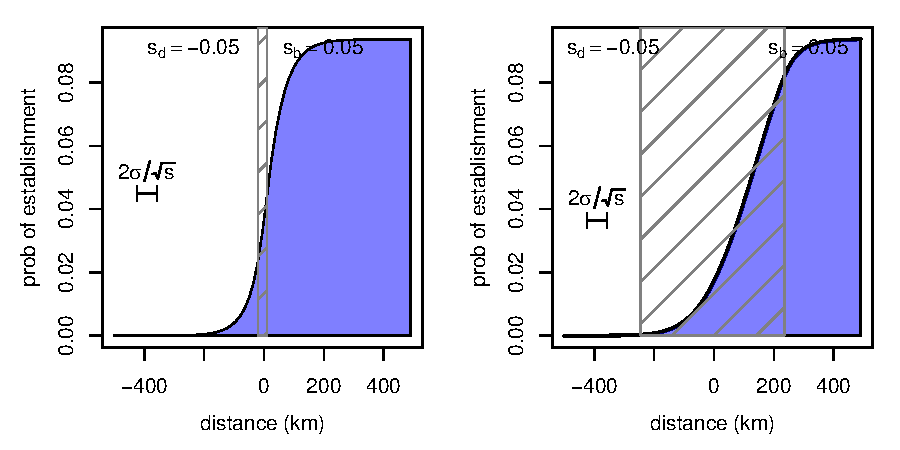
\includegraphics{prob-establishment}
    \end{center}
    \label{fig:prob_estab_calcs}
    \caption{The probability of establishment of a new mutant allele as a function of distance from the edge of the region where it is beneficial,
    in an abrupt transition (left) and a gradual transition (right).
    The allele is deleterious to the left and beneficial to the right (with selection coefficients $\mp .05$ respecively);
    and the selection coefficient interpolates linearly between these in the central shaded region.
    The number of offspring is Poisson.
    The underlying landscape has demes every 15km and a migration rate of 0.5 between neighboring demes;
    the probability was found by numerically solving the equation for the probability of establishment of a multi-type branching process.
    }
\end{figure}


%%%%%%%%%
\section{Simulations of a patchy environment}
\label{apx:patchy_sims}

Describe sims.

Argue that $C=0.5$ is a reasonable number.

\begin{figure}[ht!]
    \begin{center}
        % made in patchy-sim-writeup-plots.R
        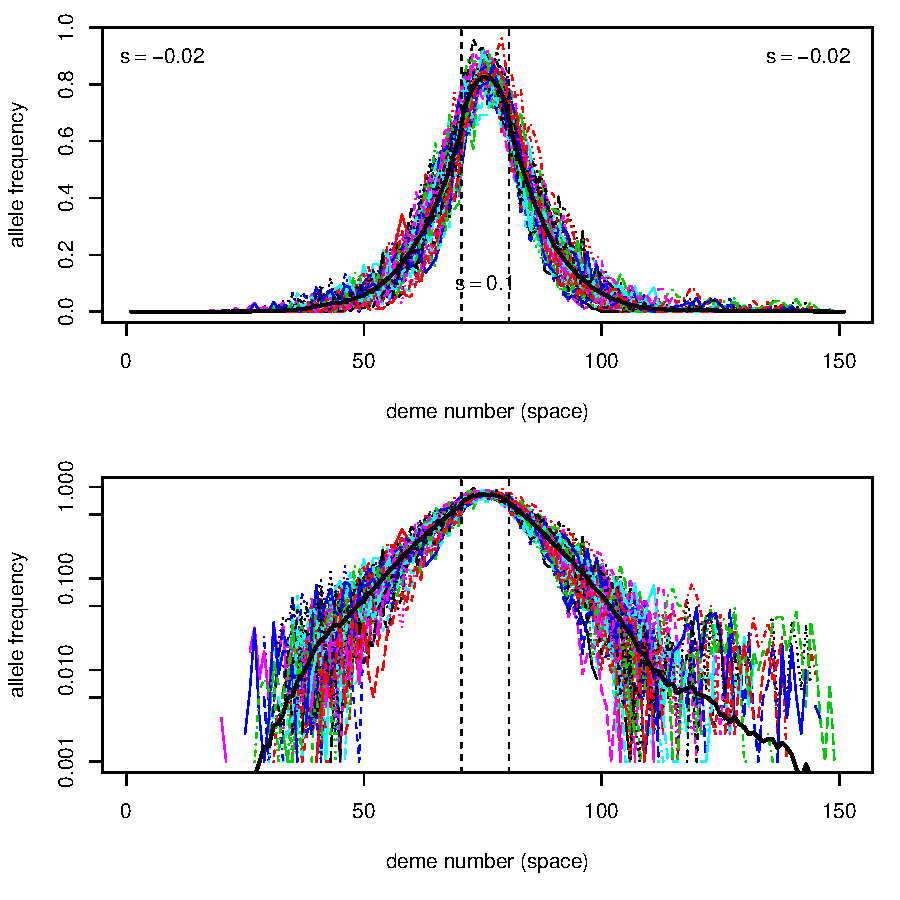
\includegraphics{example-equilibrium}
    \end{center}
    \label{fig:example_equil}
    \caption{
    Snapshots of a simulation of allelic frequency dynamics around a patch where the allele is beneficial:
    the focal allele is benefical in the middle region and deleterious outside.
    The dynamics were simulated for 10000 generations across demes with 1000 individuals in each
    and random dispersal to nearby demes with a mean dispersal distance of $\sigma \approx 2$ demes.
    Colored lines show allele frequencies across space in 50 uniformly spaced generations;
    the solid line shows the mean across all generations.
    Below is the same plot, except on a log scale.
    }
\end{figure}


%%%%%%%%%%%%
\section{The equilibrium frequency}
\label{apx:eqfreq}

One route to the ``equlibrium frequency'' of the allele outside the range where it is advantageous is as follows;
see \citet{slatkin1973geneflow} or \citet{barton1987establishment,pollak1966survival} for other arguments in this case, 
or \citet{etheridge2000introduction} or \citet{dawson1993measurevalued} for general theory used below.
Suppose that the population is composed of a finite number of small demes of equal size $N$ arranged in a regular grid,
and that selection (for or against) the allele is given by the function $s(x)$, with $x$ denoting the spatial location.
Each individual at location $x$ reproduces after a random lifetime,
dying and giving birth in the same deme to a random number of offspring with distribution given by $X$;
each offspring migrates independently to a new location chosen randomly from the distribution given by $x+R$,
where they replaces a randomly chosen individual.
If $x+R$ is outside of the range, then they perish.
Each individual's reproduction time is exponentially distributed, 
the reproduction rate is 1 if it carries the original allele, or with rate $1+s(x)$ if it carries the mutant allele.
Suppose that the number of offspring $X$ has mean $\mu$; the variance of $X$ will not enter into the formula.
Also suppose that the migration displacement $R$ has mean zero and variance $\sigma^2$;
if we are in more than one dimension, we mean that the components of the dispersal distance are uncorrelated
and each have variance $\sigma^2$.
We also assume that the distribution of $X$ makes the associated random walk irreducible and aperiodic.

Let $\Phi^N_t(x)$ be the proportion of mutant alleles present at location $x$ at time $t$,
and $\Phi_t(x)$ the process obtained by taking $N \to \infty$ (which we assume exists).
Denote by $\delta_x$ a single unit at location $x$, so that e.g.~$\Phi^N_t + \delta_x/N$
is the configuration after a mutant allele has been added to location $x$.
For $0\le \phi \le 1$, we also denote by $\bar X_\phi$ the random number of mutant alleles added if $X$ new offspring carrying mutant alleles
replace randomly chosen individuals in a deme where the mutant allele is at frequncy $\phi$ (i.e.~hypergeometric with parameters $(X,\phi)$);
similarly, $\widetilde X_\phi$ is the number lost if the new offspring do not carry the allele (i.e.~hypergeometric with parameters $(X,1-\phi)$).
(We like to think of $\Phi^N_t$ as a measure, but it does not hurt to think of $\Phi^N$ as a vector;
we aren't providing the rigorous justification here.)
Then we know that for any sufficiently nice function $f(\Phi)$ that
\begin{align} \label{eqn:discrete_generator}
  \begin{split} \frac{\partial}{\partial t} \E\left[ f(\Phi^N_t) \right] 
  &= N \sum_x \left\{ \E\left[ (1+s(x+R)) \Phi^N_t(x+R) \left( f\left(\Phi^N_t + \frac{\bar X_{\Phi_t(x+R)}}{N}\delta_{x}\right) - f(\Phi^N_t) \right) \right] \right. \\
     & \qquad  \qquad \left. {} + \E\left[ \left(1-\Phi^N_t(x+R)\right) \left( f\left(\Phi^N_t - \frac{\widetilde X_{\Phi_t(x+R)}}{N}\delta_{x}\right) - f(\Phi^N_t) \right) \right] \right\}  \end{split} \\
     &= \mu \sum_x \E\left[ \left(\partial_{\phi(x)} f(\Phi_t) \right) \left\{ \Phi_t(x+R) - \Phi_t(x) + s(x+R) \Phi_t(x+R) (1-\Phi_t(x)) \right\} \right] + O\left(\frac{1}{N}\right).
\end{align}
In the final expectation, $R$ and $\Phi$ are independent.
This follows by taking first-order terms in $1/N$ in the Taylor series for $f$, 
and the fact that $\E[\bar X_\phi] = \phi \mu$ and $\E[\widetilde X_\phi] = (1-\phi)\mu$.
We can see two things from this:
First, since this is a first-order differential operator, the limiting stochastic process $\Phi$
is in fact deterministic (check by applying to $f(\Phi) = \Phi(x)^2$ to find the variance).
Second, if we want to rescale space as well to get the usual differential equation, 
we need to choose $\var[R]=\sigma^2$ and $s(x)$ to be of the same, small, order; 
this is another way of seeing that $\sigma/\sqrt{s}$ is the relevant length scale.
More concretely, suppose that the grid size is $\epsilon \to 0$, 
that $\var[R] = (\sigma \epsilon)^2$, and that $s(x)/\epsilon \to \gamma(x)$,
and suppose that $\Phi_t(x)$ is deterministic (and sufficiently differentiable) and let $\xi(t,x) = \Phi_{t/\epsilon}(x)$;
then the previous equation with $f(\Phi) = \Phi(x)$ converges to the familiar form:
\begin{align}
  \label{eqn:derived_fkpp}
  \partial_t \xi(t,x) = \mu \left( \frac{\sigma^2}{2} \sum_{k=1}^d \partial_{x_k}^2 \xi(t,x) + \gamma(x) \xi(t,x) (1-\xi(t,x)) \right) .
\end{align}
Here we have taken first the population size $N \to \infty$ and then the grid size $\epsilon \to 0$;
we could alternatively take both limits together, but not if $\epsilon$ goes to zero too much faster than $N$ grows.
One reason for this is that at finite $N$,
the process $\Phi_t$ is an irreducible, aperiodic finite-state Markov chain with absorbing states at 0 and 1;
therefore, the inevitable outcome is extinction of one type or another,
which is not the regime we want to study.

We are interested in the equilibrium frequency,
i.e.\ the mean frequency of the selected allele at migration-selection equilibrium.
The frequency $\phi(x)$ at location $x$ solves
\begin{align}
  \label{eqn:general_phi}
  \frac{\sigma^2}{2} \sum_{k=1}^d \partial_{x_k}^2 \phi(x) + \gamma(x) \phi(x) (1-\phi(x)) = 0 
\end{align}

%%%%%%%
\section{The exact solution to the equilibrium frequency}
\label{apx:elliptic_integrals}

Here we describe how to solve \eqref{eqn:derived_fkpp} in one dimension,
i.e.\ the Fisher-KPP equation with varying selection.
Let $p(t,x)$ be the proportion of the allele under spatially varying selection $s(x)$ in one dimension,
so that 
\[
\partial_t p(t,x) = \frac{\mu}{2} \sigma^2 \partial_x^2 p(t,x) + \mu s(x) p(t,x) (1-p(t,x)) .
\]
The stable distribution $\phi(x) = \lim_{t\to\infty} p(t,x)$ then solves
\begin{align} \label{eqn:definingphi}
    \partial_x^2 \phi(x) = - 2 s(x) \phi(x) (1-\phi(x)) /\sigma^2,
\end{align}
with appropriate boundary conditions.
First rescale space by $\sigma/\sqrt{2}$ so the $\sigma^2/2$ term dissappears.
If we now assume that $s(x)$ is piecewise constant,
$s(x) = s_i$ for $x \in [x_i,x_{i+1})$, with $x_0=-\infty$ and $x_{n+2}=\infty$,
then the equation is integrable: if we multiply through by $2\partial_x \phi(x)$ and integrate, then we get that
\begin{align} \label{eqn:conservation}
    ( \partial_x \phi(x) )^2  &= - \int^{x} 2 s(x) \phi(x) (1-\phi(x)) \partial_x \phi(x) dx \\
        &= - s_i \phi(x)^2 \left( 1 - \frac{2}{3} \phi(x) \right) - K_i \quad \mbox{for } x \in [x_i,x_{i+1}) ,
\end{align}
if we define
\begin{align} 
  K_i = - s_i \phi(x_i)^2 \left( 1 - \frac{2}{3} \phi(x_i) \right) - ( \partial_x \phi(x_i) )^2  .
\end{align}
For ease of reference, we define
\[
        V_i(\phi) = s_i \phi^2 \left( 1 - \frac{2}{3} \phi \right) + K_i .
\]
Note that $V_i'(0)=V_i'(1)=0$, that $V_i(0)=K_i$ and $V_i(1) = K_i+s_i/3$.  
We will always have that $V(\phi) \le 0$.
(We have then that $\partial_x^2 \phi = - \partial_\phi V(\phi)$, the equation of motion of a particle in potential $V$.
Also note that this implies ``conservation of energy'', i.e.\ $( \partial_x \phi(x) )^2 + V(\phi(x))$ is constant.)
Rearranging, we get that $dx = d\phi / \sqrt{-V(\phi)}$, so where $\phi(x)$ is monotone, the inverse is
\[
    x(\phi) = x(\phi^*) \pm \int_{\phi^*}^\phi \frac{ d\psi }{ \sqrt{ -V(\psi) } } .
\]
For each $i$ then define the elliptic function
\begin{align}  \label{eqn:elliptic_function}
    F_i(\phi) = \int_{\phi_i^*}^\phi \frac{ d\psi }{ \sqrt{ -V_i(\psi) } } ,
\end{align}
where take the positive branch of the square root, and $\phi_i^*$ will be chosen later.
Then we have that
$x(\phi) - x(\phi_0) = \pm( F(\phi) - F(\phi_0))$,
or for an appropriate $x_0$,
\[
    \phi(x) = F^{-1}\left( F(\phi(x_0)) \pm (x - x_0) \right).
\]

We clearly want $\lim_{x \to \infty} \partial_x \phi(\pm x) = 0$, 
and $\lim_{x \to \infty} \phi(\pm x)$ to be zero or one depending on the sign of $s_0$ and $s_{n+1}$.
Since $(\partial_x \phi(x))^2 = -V(x)$, this implies that if $s_0<0$, then $K_0 = 0$,
while if $s_0>0$ then $K_0 = s_0/6$; and likewise for $K_{n+1}$.

We also require that $\phi(x)$ and $\phi'(x)$ are continuous.
Continuity of $\phi'(x)$ is equivalent to $V_i(x_{i+1}) = V_{i+1}(x_{i+1})$,
which we can rearrange to find an equation for $K_{i+1}$ in terms of $K_i$ and $\phi(x_{i+1})$:
\[
    K_{i+1} - K_i = (s_i - s_{i+1}) \phi(x_{i+1})^2 (1-2\phi(x_{i+1})/3) .
\]
What about the frequency at the points the selection changes, $\phi(x_i)$?  
Well, if $\phi(x)$ is monotone on $[x_i,x_{i+1})$ then we can without loss of generality take $\phi_i^*=0$ or $1$ depending on the sign of $s_i$.
Otherwise, let $\phi_i^*$ be the (unique) root of $V_i$ in $[x_i,x_{i+1})$, so $V_i(\phi_i^*)=0$.
In this case, $\phi_i^*$ is the maximum or minimum of $\phi$ in the interval:
if $s>0$, then $\phi_i = \max\{ \phi(x) : x \in [x_i,x_{i+1})\}$. 
Recall we defined $F_i$ using $\phi_i^*$; now using the fact that $\phi$ is monotone with the opposite sign on either side of $\phi_i^*$,
$x_{i+1} - x_i = F_i(\phi(x_{i+1})) - F_i(\phi_i^*) + F_i(\phi(x_{i})) - F_i(\phi_i^*)$,
and that $F(\phi_i^*) = 0$,
we know that the length of the $i$th stretch is
\[
    x_{i+1} - x_i = \pm \left( F_i(\phi(x_i)) + F_i(\phi(x_{i+1})) \right).
\]
Note that all the $\pm{}$'s are easily relatable to the signs of $s_i$.
If we knew $\phi(x_1)$ and $\phi'(x_1)$, then we'd be able to solve the equations for $\phi(x_i)$ and $K_i$ recursively upwards.
In some cases, such as \citet{slatkin1973geneflow}, we can infer $\phi(0)$ and $\partial_x \phi(0)$ by spatial symmetry.
In other cases, we are only given $\phi(-\infty)$ and $\phi(\infty)$, and have to work inwards from the ends.

We are interested in the following case:
\[
    s(x) = \begin{cases}
        +s_b \qquad \mbox{for } |x|<\epsilon \\
        -s_d \qquad \mbox{for } x<-\epsilon \; \mbox{or}\; \epsilon \le x \le R \\
        -s_* \qquad \mbox{for } R < x < R+2\epsilon \\
        -s_d \qquad \mbox{for } x>R+2\epsilon .
    \end{cases}
\]
We can solve the case with $s_* = s_d$, since $\phi'(0) = 0$ (as done implicitly in \citet{slatkin1973geneflow}).
We should be able to argue that if $R$ is large then the value of $s_*$ won't make much difference.

\subsection{Doing the integrals}

An important ingredient in the above method is the integral \eqref{eqn:elliptic_function},
to which a method for solving the Korteweg-de Vries equation can be applied \citep{NEQwiki}.
Recall that $V_i(\phi) =  s_i \phi^2(1-2\phi/3) + K_i$, with $K_i = V_i(0)$ chosen to match $V$ at the boundaries;
since we're just working within an interval with $s$ constant, we can rescale space by $\sqrt{2 s_i}/\sigma$,
so that $s$ and $\sigma$ drop from the equation.
We then want to integrate
\[
    \int \frac{ d\phi }{ \sqrt{-V(\phi)} } = 
         \int \frac{ d\phi }{ \sqrt{ \phi^2 (1-2\phi/3) + K } } ,
\]
over a domain where $V$ is always negative.
Let $\phi^2(1-2\phi/3)+K = (\alpha-\phi)(\phi-\beta)(\phi-\gamma)$,
and change variables first to $y^2=(\alpha-\phi)$, 
and then to $x = y/\sqrt{\alpha-\beta}$, so that
\begin{align*}
    \frac{ d\phi }{ \sqrt{ \phi^2 (1-2\phi/3) + K } } 
        = \frac{ - 2 dy }{ \sqrt{ (\alpha-\beta-y^2) (\alpha-\gamma-y^2) } } \\
        = \frac{ - 2 dx }{ \sqrt{\alpha-\gamma} \sqrt{ (1-x^2) (1-S^2 x^2) } } ,
\end{align*}
with $S^2 = (\alpha-\beta)/(\alpha-\gamma)$.
Now Jacobi's incomplete elliptic integral of the first kind is defined by
\[
    F(x;k) = \int_0^x \frac{dt}{\sqrt{ (1-t^2)(1-k^2t^2) }} ,
\]
and the Jacobian elliptic function $\sn(x;k)$ is the inverse: $F(\sn(x;k);k) = x$.
As $k \to 0$, $\sn(x;k) \to \sin(x)$, while as $k \to 1$, $\sn(x;k) \to \sinh(x)$.

Presumably, this gets the same answer as Monty, who finds that in his solvable cases,
for $x$ in the last interval (which ends in $\infty$), that
\begin{align*}
    \phi(x) &= \frac{3}{2}\left( 1 - \tanh^2 ( x \sqrt{2s} / 2 \sigma + C ) \right) \\
        &\simeq C' \exp\left( - \frac{ x \sqrt{2s} }{ \sigma } \right) .
\end{align*}
% Indeed, as $\phi \to 0$, we have approximately $\phi' = \frac{ \sqrt{s} }{ \sigma } \phi$.  % huh????



%%%%%%%%%%
\section{Asymptotics for the equilibrium frequency}
\label{ss:asymptotic_freq}

We provide the above discussion on exact solutions mostly for completeness;
in practice, we use asymptotics of the solutions.
These are furthermore available for $d=2$, where we have no analytic solutions.
In $d=2$ (and higher) dimensions, we are more interested in the mean frequency at a given distance $r$ from a patch.
Suppose therefore that the patch is radially symmetric,
and that the allele is uniformly deleterious outside of some radius $r_0$
(in the notation above, $\gamma(x) = -s_m$ for $|x|>r_0$).
Then, denoting by $\phi(r)$ the mean occupation frequency at distance $r$ at equilibrium,
the polar form of the Laplacian in $d$ dimensions translates equation \eqref{eqn:general_phi} to
\begin{align}
  \label{eqn:radial_phi}
  \frac{\sigma^2}{2} \partial_{r}^2 \phi(r) + \sigma^2\frac{d-1}{2r} \partial_r \phi(r) &= s_m \phi(r) (1-\phi(r)) \quad r>r_0 , \\
  \phi(r_0) = \phi_0 , \qquad \phi(r) \ge 0 .
\end{align}
We wish to find the asymptotic behavior of $\phi$ for large $r$.
The argument can likely be extended to patches that are not radially symmetric.

The solution with $d=2$ is $C Y_0(ir) \sim C e^{r}/\sqrt{2 \pi r}$ (G\&R 8.451.2).



%%%%%%%%%%
\section{The probability of establishment}
\label{ss:prob_estab}


In the main text we have made use of two decompositons of the spatial branching process
to approximate in two different ways the rate of establishment of migrant alleles.
Here we make the relationship more formal.
The decompositions use a similar idea to that found in \citep[section D.12]{athreyaney},
where a supercritical branching process is decomposed into individuals whose families eventually die out
and those having infinite lines of descent.
We also note that the approximations fall generally in the realm covered by \citet{aldouspoissonclumping}.

Consider a discrete-time branching process $Z_t$ with spatial motion and offspring distribution depending on spatial location.
Suppose that the offspring distribution for an individual at location $x$ is distributed as $X_x$.
We can record the state of the process simply as the list of locations of individuals:
$Z_t = (x_1, \ldots, x_{N(t)})$ means that there are $N(t)$ individuals alive at $t$, at locations $x_1, \ldots, x_{N(t)}$.
We can construct the process iteratively: given $Z_t$,
we sample first the number of offspring of each, and then the locations the offspring migrate to.
Concretely, given $Z_{t} = (x_1, \ldots, x_{N(t)})$,
first let $X_1(t),\ldots,X_{N(t)(t)}$ be independent random draws from the offspring distribution,
with $X_k(t)$ having distribution $X_{x_k}$.
The number of new offspring is $N(t+1) = \sum_{k=1}^{N(t)} X_k(t)$,
and we can sample their locations independently given the location of their parent to obtain $Z_{t+1}$.
Note that the genealogy is implicitly recorded:
the parent of the $k^\mathrm{th}$ individual at time $t$ is
the $a(k,t) = \min\{ \ell : \sum_{j=1}^\ell X_j(t-1) \ge k \}$-th individual at time $t-1$.
It will be useful to extend this to more distant ancestors:
let $a_1(k,t) = a(k,t)$ and recursively define $a_m(k,t) = a(a_{m-1}(k,t),t-m+1)$, as long as $m\le t$.

We want to find (approximations to) $p(x)$, the probability that a branching process beginning with a single individual at $x$ does not die out. 
(In other words, $p(x) = \P\{ N(t) = 0 \; \mbox{for some}\; t>0 \; \vert \; Z_0 = (x) \}$.)
We assume that the mean number of offspring $\E[X_x]$ is only greater than one for $x \in A$ (``the patch''),
and so the process can only establish if some offspring eventually get to the patch (with probability one).

The second decomposition we use is simpler, only conditioning on the number of individuals who ever reach the patch.  
Let $\calE = \{(t_i,k_i)\}$ be the times and indices of individuals who are in the patch but none of whose ancestors have been --
i.e.\ $(t,k) \in \calE$ iff $x_k(t) \in A$ and $a_m(k,t) \notin A$ for all $1\le m \le t$.
If we remove these individuals (and their offspring), the resulting branching process has mean number of offspring less than or equal to 1 everywhere,
so there are a finite number of such individuals with probability one (the process dies out).
Therefore, the probability that the process dies out is then the probability that the families descending from each individual in $\calE$ dies out.
By independence of different offspring, this is
\begin{align}
  1-p(x) = \E\left[ \prod_{(t,k) \in \calE} (1-p(x_k(t))) \; \vert \; Z_0 = (x) \right] .
\end{align}
Above, we make the approximation that $p(x_k(t)) \approx p_e$,
the probability of establishment ignoring the possibility of migrating outside the patch.
In this case,
\begin{align}
  p(x) \approx \E\left[ p_e^{|\calE|} \; \vert \; Z_0 = (x) \right] .
\end{align}
Here $|\calE|$ is the ``size of the family that reaches the patch'';
in section \ref{ss:haplotype_length} we estimated the probability that any of the family reaches the patch
and argued that the distribution of $|\calE|$ is given by $K$,
the size of the subcritical branching process conditioned on still being alive.


The first approximation uses a similar trick, but rather than treating all individuals migrating into the patch
as an opportunity for establishment,
we couple the branching process to a strictly subcritical branching process
that produces extra offspring, each of which provides an opportunity for establishment.
To this end, suppose that the offspring distribution off the patch is given by $X'$ (so $X_x \deq X'$ for $x \notin A$),
and the offspring distribution within the patch stochastically dominates $X$,
i.e.\ $\P\{X_x\ge n\} \ge \P\{X'\ge n\}$ for all $x\in A$ and $n \ge 0$.
Stochastic domination implies that we can \emph{couple} any instance of $X_x$ with one of $X'$ and a remainder --
i.e.\ jointly construct an $X'$ and a $Y_x$ such that $X_x = X' + Y_x$,
and that $Y_x$ also takes values in the nonnegative integers.
We can therefore modify the construction of the branching process above,
so that $X_k(t) = X_k'(t) + Y_k(t)$, where $X_k'(t) \deq X$ and $Y_k(t) \deq Y_{x_k(t)}$.
We can define a \emph{core} branching process $Z'$ using the $X'$, which will be finite (since $\E[X']<1$).
Formally, say that the first $X_k'(t)$ offspring of the $(t,k)^\mathrm{th}$ individual are ``core'' offspring,
denoted by $\calC_t = \{ (t,k) \; : \; 0 \le k - \sum_{j<\ell} X_j(t) \le X_\ell'(t) \; \mbox{for some}\; 1 \le \ell \le N(t) \}$;
and define $Z'$ as the core individuals whose ancestors are all ``core'' as well,
i.e.\ $Z'_t = \{ x_k \in Z_t \; : \;  a_m(k,t) \in \calC_{t-m} \; \mbox{for all}\; 0 \le m \le t\}$.
The boundary analogous to above in the first computation is then the non-core offspring of core individuals;
denote the times and indices of these by $\partial \calC$,
so that $(t,k) \in \partial \calC$ iff $(t,k) \notin \calC_t$ and $a(k,t) \in \calC_{t-1}$.
We can now use this as above to compute the probability of establishment beginning from a single individual:
\begin{align}
  1-p(x) = \E\left[ \prod_{(t,k) \in \partial\calC} (1-p(x_k(t))) \; \vert \; Z_0 = (x) \right] ,
\end{align}
but this is less helpful, as the distribution of $\calC$ is harder to get at.

However, recall the actual problem at hand.
Roughly speaking, we approximate the process of colonization of the new patch by migrants from an established patch
by imagining that the established patch sends out migrants, and that each of these acts as an independent branching process,
at least in the region of the new patch.
We can suppose that migrant families appear at some rate, say, midway between the patches, and far enough from the original one that we can ignore it,
and leave the precise distribution of their appearance unspecified
We can decompose each of these branching processes as above into ``core'' and ``extra'',
so that the point in time of ``establishment'' is well-defined:
the time $\tau$ of first appearance of an ``extra'' offspring with infinite line of descent.
Given that establishment has not yet occurred by $t$, 
and the combined state of the core process $Z'_t$,
then the mean number of establishment events occurring at time $t$ is $\sum_{x \in Z'_t} p(x) \E[Y_x]$.

If establishment events were independent and sufficiently rare,
the influx of branching processes begain long enough ago that $Z'$ was at stationarity
with $z_A := \E[ \# \{ (x,t) \in Z'_t : x \in A \} ]$,
and we again approximate $p(x) \approx p_e$,
then we would have that 
\begin{align}
  \P\{\tau>t\} \approx \exp\left\{ - t z_A \E[Y_x] p_e \right\} ;
\end{align}
in our case, $\E[Y_x] \approx (s_p+s_m)$ and $p_e \approx 2 s_p/\xi^2$,
so $\tau$ is approximately exponentially distributed with rate $ 2 z_A (s_p+s_m) s_p/\xi^2 $.
We can get $z_A$, the occupation density without the new patch, 
directly by integrating the expression~\eqref{eqn:eqfreq} over the patch.

In obtaining an exponential distribution, we have assumed effectively that establishment events
are independent of each other.
This will not be strictly true, since an establishment implies that a family of migrants are present in the patch,
and hence others may produce offspring with infinite lines of descent at a similar time.
The mean total family size of an allele with fitness $1-s_m$ (i.e.\ a subcritical branching process) is $\sum_{t \ge 0} (1-s_m)^t = 1/s_m$;
so the mean number of ``extra'' offspring is $1+s_p/s_m$.
Establishment events are correlated to the extent that single such families give rise to multiple establishment events,



% We will record the state of the branching process as a finite point measure,
% so that if there are $n$ individuals alive at $t$, at locations $x_1, \ldots, x_n$,
% then $Z_t = \sum_{k=1}^n \delta_{x_k}$, and we write $Z_t(A) = \sum_{k=1}^n \bone_{x_k \in A}$ for the number of individuals in a set $A$.

%%%%%%%%%%%
\section{Patchy selection} 
\label{ss:discretedemes}

We have been working in a continuous model of geographic space; 
in this section we move to a discrete model of isolated populations exchanging rare migrants,
but in section \ref{ss:patchyspace} discuss how a model with {\em patchy} selection can be approximated by such a discrete model.

Suppose now that we have a set of $L$ discrete populations of individuals that may reproduce or migrate,
and that migration and mutation are rare, so that the waiting times until either event is approximately exponential.
Suppose that for each pair of populations, labeled $i$ and $j$, the mean number of migrants that travel from $i$ to $j$ per generation
is $M_{ij}$ and that the mean number of new mutations appearing in population $i$ per generation is $\mu_i$.

{\tt Include cartoon here.}

If we suppose that fixation occurs on a faster time scale than mutation or migration,
so that it is very unlikely that two different migrants or mutants begin to fix locally in the same population,
then we can treat the process of extinction or local fixation as instantaneous 
(a limit previous studied by \cite{Slatkin:81}).
In this limit we may also ignore swamping effects of inmigration of nonmutant alleles.

In this case, we have the following picture.
The population at first starts out with no selected alleles. 
At some later time point suppose that there are $T$ different alleles present in the population, 
that the $k^\mathrm{th}$ allele is occupying demes $\{i^k_1, \ldots, i^k_{n_k}\}$, for $1\le k \le T$.
Let $I$ denote the set of all adapted demes, 
and let $J = \{j_1, \ldots, j_\ell\}$ denote the demes that have not yet adapted, with $\ell = L - \sum_k n_k$.
Then we are assuming that two types of event can happen which could change the state:
either at rate $\mu_j p_f$, an unadapted deme $j$ produces a new mutant, which fixes in this deme;
or at rate $M_{ij} p_f$, an adapted deme $i$ sends a migrant to unadapted deme $j$, which fixes in that deme.
Therefore, under these assumptions, the probability of fixation $p_f$ (and hence the selection coefficient)
only enter as a time scaling: for instance,
if we define $R = \sum_{j \in J} \left( \mu_j + \sum_{i \in I} M_{ij} \right)$,
then the total rate of such events is $p_f R$.
The probability that the next event results in, say, adaptation of deme $j$
is 
\[
 \left( \mu_j + \sum_{i \in I} M_{ij} \right) / R,
\]
and the probability that deme $j$ adapts through migration from deme $i$, given that deme $j$ is the next to adapt, is
$M_ij / R$,
while the probability that it adapts through a new mutation is $\mu_j / R$.

The main point here is that the final pattern,
and hence the likely extent of parallel adaptation,
is independent of the strength of selection.
This is in contrast to the continuous case, however, this observation is dependent on the assumption of weak migration
and fails to hold if different migrant lineages interact.
This can be viewed as a continuous-time Markov process XXX.
Explicit solutions are not available in the general case,
but if we specialize to a completely symmetric model (i.e.\ the ``island'' model),
then the mathematical picture is a pretty one.

\subsection{Symmetric patches}

Indeed, suppose that migration and mutation are symmetric: $M_{ij}=m$ and $\mu_j = \mu$ for all $j$ and $i\neq j$.
Suppose at some time the $k^\mathrm{th}$ allele is occupying $n_k$ demes, 
with $n = \sum_k n_k < L$.
Then at rate $(L-n) N \mu p_f + n (L-n) N m p_f$,
either a migration or mutation event happens.
With probability $\mu/(\mu + n m)$, it is a mutation,
and a new deme is randomly chosen and assigned a new allele.
With probability $n_k m / (\mu + n m)$,
the $k^\mathrm{th}$ type sends a successful migrant to a randomly chosen new island,
which is assigned the $k^\mathrm{th}$ allele.

This process is a continuous-time version of the ``Chinese restaurant process''
described in \citet{aldous1985exchangeability} and \citet{pitman1995partitions},
and so the final partition of types across demes has the Ewens sampling distribution with parameter $\mu/m$.
Again note that the selection coefficient, which is implicit in the probability $p_f$,
does not enter into the final distribution.

Now we can compute most properties we might want about the process.
For instance, the expected number of distinct mutational origins is
\begin{equation}
    \E\left[ \mbox{ \# of independent mutations } \right] = 
            1 + \frac{\mu}{m} \sum_{k=2}^L \frac{1}{k+(\mu/m)}. \label{discrete_expected}
\end{equation}
The probability that there is only a single successful mutation is
\begin{equation}
\P \left\{ \mbox{only one mutational origin} \right\} = 
            \prod_{k=1}^{L-1} \frac{ k }{ k+(\mu/m)} .
\end{equation}
More generally, suppose we sample a single deme, and are interested in the total number of demes $S$
(including the sampled one) that share the same fixed mutation as our sampled deme.
Then $S$ has distribution
\begin{equation} \label{eqn:Sdistrn}
\P\{ S=s \} = \frac{ (s-1)! (\mu/m)^{L-s} }{ \prod_{k=1}^{L-1} (k+(\mu/m)) } .
\end{equation}
Furthermore, if $L$ is large, then $S/L$ has probability density approximately
\begin{equation} \label{eqn:betadistrn}
   (\mu/m) (1-x)^{(\mu/m)-1}
\end{equation}
namely, is a $\mathrm{Beta}((\mu/m), 1)$ distribution--- see \cite{donnelly-joyce} and \cite{permanPitmanYor92}.

% In Figure \ref{fig:discbyratio} we plot mean number of types and size (number of demes occupied) of a sampled type,
% for a model with 20 interconnected demes, across different parameter values.  
% This indicates that we need the population-scaled mutation and migration rates to be within a factor of about 100 of each other for parallel adaptation to leave an interesting pattern. If migration is faster, then a single type is likely to take over, while if migration is weaker, each deme is likely to come up with its own type.

The high connectedness of the discrete deme island model means that the expected number of distinct alleles, (Equation \eqref{discrete_expected}), 
grows with the $\log$ of the number of demes. This strongly contrasts with the continuous spatial model where the local nature of dispersal means that doubling the species range will double the number of mutations expected. 
Furthermore, while in the continuous model the areas occupied by distinct mutations are similar in area, in this strong-selection discrete island model, 
only a few types tend to dominate even as the number of demes (and thus, distinct types) grows large (see Equations \eqref{eqn:Sdistrn} and \eqref{eqn:betadistrn}).

A more general model would allow migration only along edges of some graph connecting the demes.
In the low migration limit such a model still produces a partition distribution independent of the selection coefficient,
but it does not in general have the Ewens distribution.
Another extension would be to include the time alleles need to achieve an intermediate frequency,
along the lines of \citet{Navarro:03}, which would reintroduce dependence on the selection coefficient.

\texttt{XXX omit this? XXX}
We have treated the time during which the selected allele is at intermediate frequency in a deme (about $\log(\sigma^2 \rho)/s_p$ generations) as negligible, 
which ignores migration events that occur while the mutation is spreading through the population. 
we now sketch of a more realistic approximation.
For each occupied--unoccupied pair of demes, if the number of mutant alleles in the occupied deme is $n(t)>0$,
then at time $t$, migrants from the occupied deme pass the selected allele to the unoccupied deme at rate $2 n(t) m p_f(s_p)$,
while newly arisen mutants arise and fix in the unoccupied deme at constant rate $2 N \mu p_f(s_p)$.
The selected type should grow approximately as $n(t)=\exp(s(t-t_0))$.
Of course, to follow this model through, we will have to account for multiple types within a single deme and other complications,
but we can at least make a few observations.
One is that the final distribution of types is no longer independent of $s_p$, which enters through the dynamics $n(t)$.
However, it is clear that increasing the selection coefficient $s$ will decrease the number of types (independent mutational origins),
while on the other hand, increasing the deme size $N$ will increase the number of types,
and that the case presented above is at the extreme (see also \cite{Navarro:03} for deterministic approximations). 


\end{document} 
